\chapter{Automatic generator}
The automatic generator of Gr\"obner basis solvers is used to easily solve problems leading to systems of polynomial equations. These systems usually arise when solving minimal problems \cite{MinimalProblems} in computer vision. Typically, these systems are not trivial so special solvers have to be designed for concrete problems to achieve efficient and numerically stable solvers. But solvers generated for concrete problems can not be easily applied for similar or new problems and therefore the automatic generator was proposed in \cite{AutoGen}. Solvers generated by the automatic generator can be easily used to solve complex problems even by non-experts users.

The input of the automatic generator is a system of polynomial equations with a finite number of solutions and the output is a MATLAB or a Maple code that computes solutions of the given system for arbitary coefficients. One of the goals of this thesis is to improve previous implementation \cite{AutoGen} of the automatic generator to construct more efficient and numerically stable solvers.

The newest version of the automatic genenerator implemented in MATLAB can be downloaded from \cite{AutomaticGenerator}.

\section{Description of the automatic generator}
In this section we would like to briefly describe the procedure for generating solvers. The automatic generator consists of several independent modules, see Figure \ref{autogen:blockDiagram}. Since all these modules are independent, they can be easily improved or replaced by more efficient implementations. Next we describe each of these modules, full description can be found in \cite{AutoGen}.

\begin{figure}[ht]
  \centering
  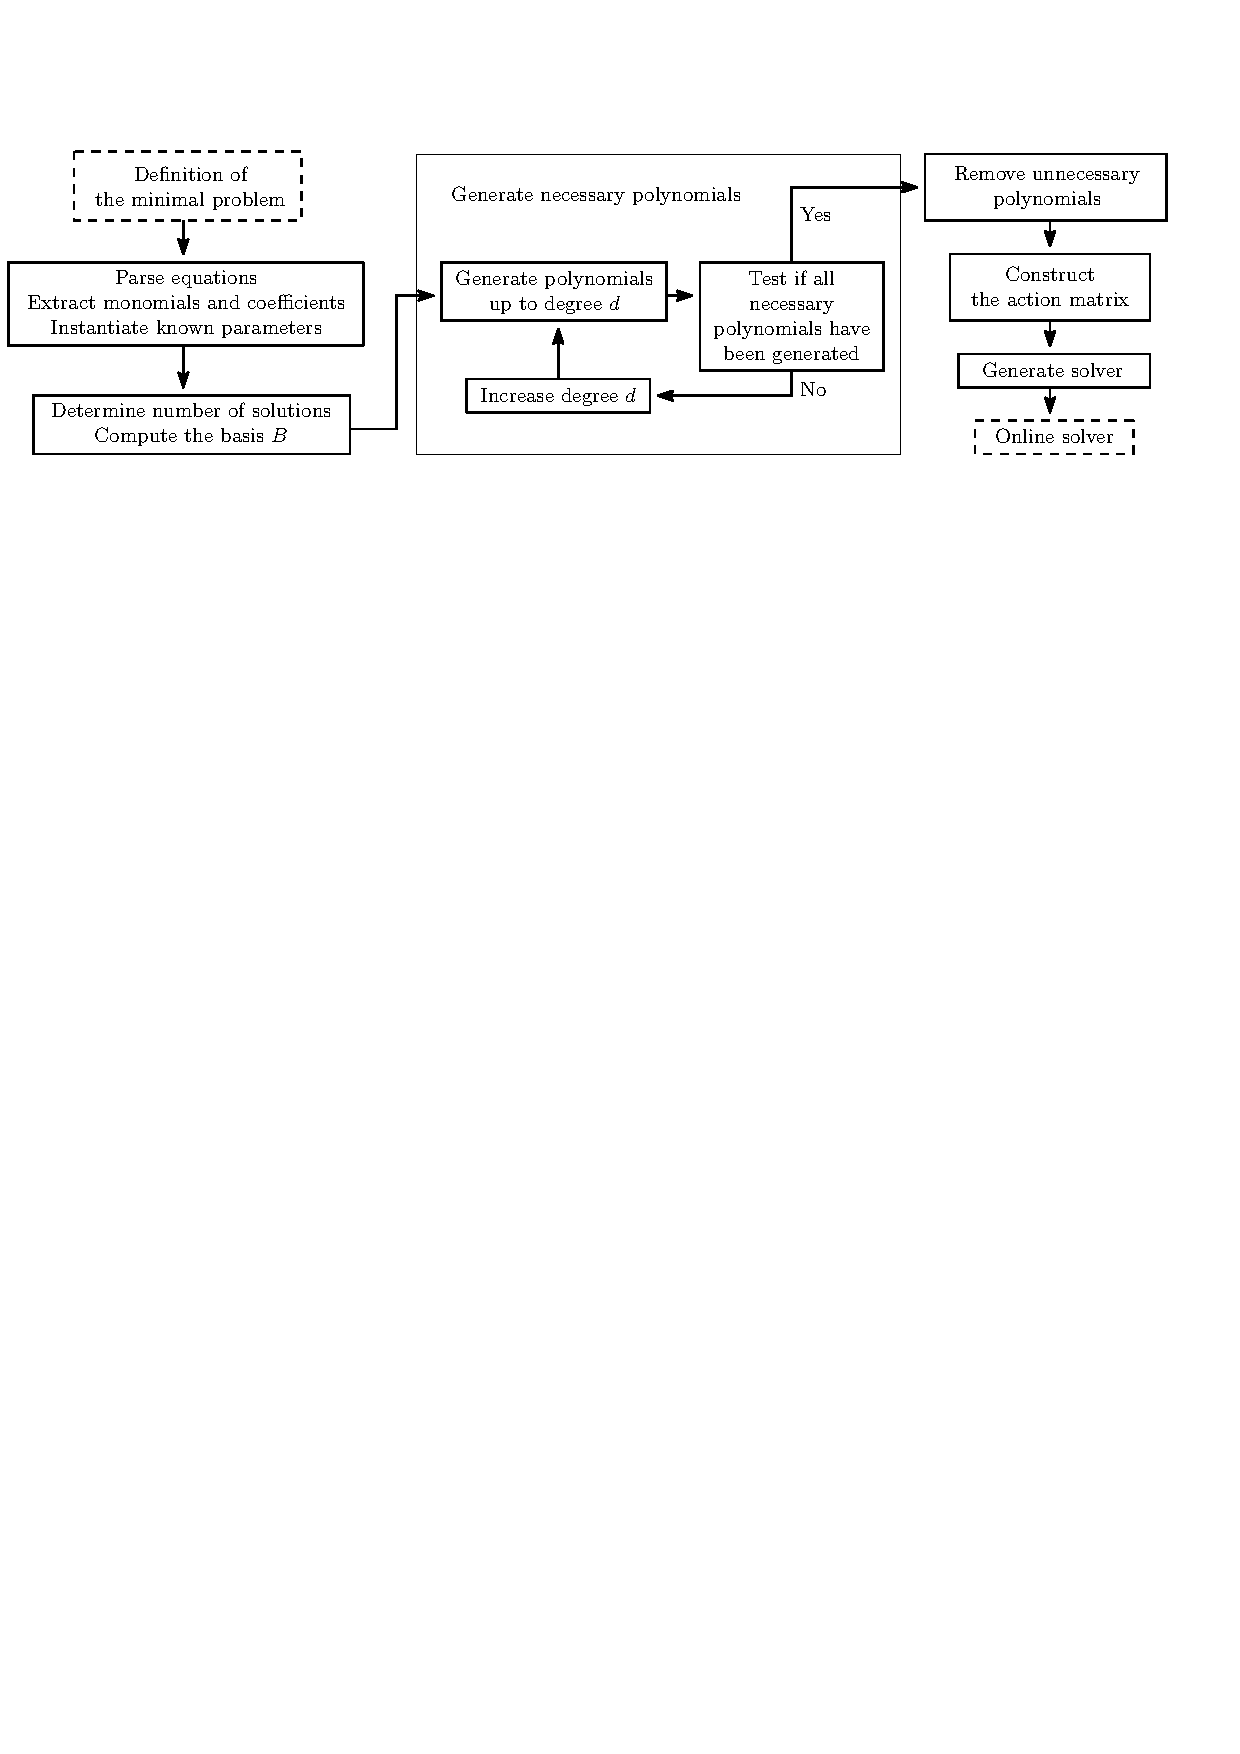
\includegraphics[width=0.95\textwidth]{AutomaticGenerator.pdf}
  \caption{Block diagram of the automatic generator}
  \label{autogen:blockDiagram}
\end{figure}

\subsection{Definition of the minimal problem}
Definitions of minimal problems are written in separate functions that are stored in the folder \texttt{minimalProblems}. Each of the definitions has to contain few necessary information about the minimal problem. First of all, the system of polynomial equations with symbolic variables and parameters has to be provided. Next we have to specify the list of unknown variables and known parameters. Optionally if we know the monomial basis $B$ of the polynomial system in advance we can specify it to save some computation time. The monomial basis $B$ is a set $\left\{m\ |\ \overline{m}^G = m\right\}$ where $m$ is a monomial and $G$ is the Gr\"obner basis of the given polynomial system. At last we have to set some settings for the automatic generator. We recommend to obtain the default settings by calling the function \textit{gbs\_InitConfig()} and only overwrite the settings we want to change. In the folder \texttt{minimalProblem} there are some examples which are self explanatory and can be used as templates to create new minimal problem definitions.

\subsection{Equations parser, Instantiating}
In the next step we have to parse the given equations, that means we extract used monomials and parameters and obtain total degrees of the polynomials. Then we instantiate each known parameter with a random number from $\mathbb{Z}_p$. We assign unique identifier to each used parameter. The reason is that we need to track the parameters through the process of adding polynomials in order to be able to restore the process in the solver generation module.

\subsection{Monomial basis $B$ computation}
We need to know the monomials basis $B$ to recognize when we have generated all polynomials that are necessary to build the action matrix. If the basis $B$ was not provided within the definition of the minimal problem we have to compute it by ourselves. Because in MATLAB there is no function or simple script to compute the basis we have to do it by calling an external software.

The most easy solution to implement is to use the Maple toolbox for MATLAB. This enables us to call Maple functions from the MATLAB environment directly. To use this option we have to set \texttt{cfg.GBSolver = @gbs\_findAlgB\_maple} in the settings of the automatic generator. Unfortunately it shows up that the symbolic toolbox provided by Maple in not compatible with the MATLAB symbolic toolbox in versions newer than R2008 so we do not recommend to use this option nowadays, but the option is still available to use on older computers.

The second implemented option is to use the algebraic geometry software Macaulay2 \cite{M2}. In the folder \texttt{gbsMacaulay} there is a template \texttt{code\_template.m2} into which we simply write the given polynomial system. This updated file is saved as \texttt{code.m2} which is executed by Macaulay2 and the results are parsed back in MATLAB. To set up this option we need to install the software Macaulay2 and set \texttt{cfg.GBSolver = @gbs\_findAlgB\_macaulay} in the automatic generator settings. A problem could be that the Macaulay2 is not easy to set up under the Windows OS. Therefore the installation file of Macaulay2 is provided within the automatic generator. The only thing that has to be done is to edit the file \texttt{calc.bat} in the folder \texttt{gbsMacaulay} and follow the instructions in the file.

Because of the modularity of the generator this part can be replaced by another function computing the monomial basis $B$.

The last option is to compute the basis $B$ in advance and set it into the definition of the minimal problem.

In the end we have check the number of solutions of the given polynomial system. If there is a finite number of solutions we can continue with the computation.

\subsection{Polynomial generator}
To be able to build the action matrix we have to generate enough polynomials such that after their reduction there will be polynomials with required leading monomials. The monomial basis $B$ tells us which leading monomials are required for the contruction of the action matrix.

In this part of the automatic generator we represent polynomials as row vectors so systems of polynomials can be represented by matrices. This representation enables us to easily multiplicate polynomials with monomials only by shifting the coefficients in the vectors or to reduce the whole polynomial systems by performing the Gauss-Jordan eliminations on the corresponding matrices.

Let $f_1, \dots, f_n$ are the polynomials from the input. Let $maxdeg$ is a maximal total degree of all polynomials $f_i$. At the beginning we put into the matrix $M$ all polynomials $\left\{m\times f_i\ |\ i = 1,\dots n;\ deg(m\times f_i) = deg(f_i),\dots, maxdeg\right\}$, where $m$ is a monomial. Now we perform the Gauss-Jordan elimination on the matrix $M$ and the result save as matrix $\tilde{M}$. Then we check if there exists a variable for which all required monomials are present as leading monomials of polynomials from $\tilde{M}$. If we find such a variable we can continue with the construction of the action matrix for the found variable. If not we have to add more polynomials to the matrix $M$. We increment $maxdeg$ by one and add all polynomials $\left\{m\times f_i\ |\ i = 1,\dots n;\ deg(m\times f_i) = maxdeg\right\}$ to the matrix $M$. Then we continue with the elimination and with the checking the action matrix requirements as written above. We repeat these steps until all required polynomials are generated so the action matrix can be built.

In this whole process we need to keep track how the matrix $M$ was built. Recall that each coefficient of the polynomials $f_i$ has unique identifier assigned in the equations parser. Because the whole matrix $M$ contains only the polynomials $f_i$ or their multiples with monomials therefore in the matrix $M$ appear only the coefficients from the polynomials $f_i$. We just have to keep the positions of the coefficients. This is done by matrix $M_c$. The matrix $M_c$ is built in same time as the matrix $M$ by this way: if we put a coefficient into the matrix $M$ we also put the corresponding indentifier to the matrix $M_c$ at the same possition. The matrix $M_c$ enables us to recover the process of polynomials generation in the code generator module.

\section{Reimplementation}

\section{Multiple eliminations solver}

\section{Removing unnecessary polynomials}

\section{Matrix partitioning}

\section{F4 strategy}
